\documentclass[problem]{mcs}

\begin{pcomments}
  \pcomment{CP_prerequisite_relation}
  \pcomment{from: F10.cp4w, revised from S09.cp3r by ARM}
\end{pcomments}

\pkeywords{
  relations
  scheduling
  partial_orders
}

%%%%%%%%%%%%%%%%%%%%%%%%%%%%%%%%%%%%%%%%%%%%%%%%%%%%%%%%%%%%%%%%%%%%%
% Problem starts here
%%%%%%%%%%%%%%%%%%%%%%%%%%%%%%%%%%%%%%%%%%%%%%%%%%%%%%%%%%%%%%%%%%%%%

\begin{problem} \mbox{}  %LaTeX artifact to position the table

\begin{center}
\begin{tabular}{|l|l|}
\hline
Direct Prerequisites & Subject\\ \hline
 18.01 & 6.042\\ \hline
 18.01 & 18.02\\ \hline
 18.01 & 18.03\\ \hline
 8.01  & 8.02\\ \hline
 8.01  & 6.01\\ \hline
 6.042 & 6.046\\ \hline
 18.02, 18.03, 8.02, 6.01 & 6.02\\ \hline
 6.01, 6.042 & 6.006\\ \hline
 6.01 & 6.034\\ \hline
 6.02 & 6.004\\ \hline
\end{tabular}
\end{center}

\bparts

\ppart\label{prereqtable} For the above table of MIT subject
prerequisites, draw a diagram showing the subject numbers with a line
going down to every subject from each of its (direct) prerequisites.

\begin{solution}\mbox{}

\begin{center}
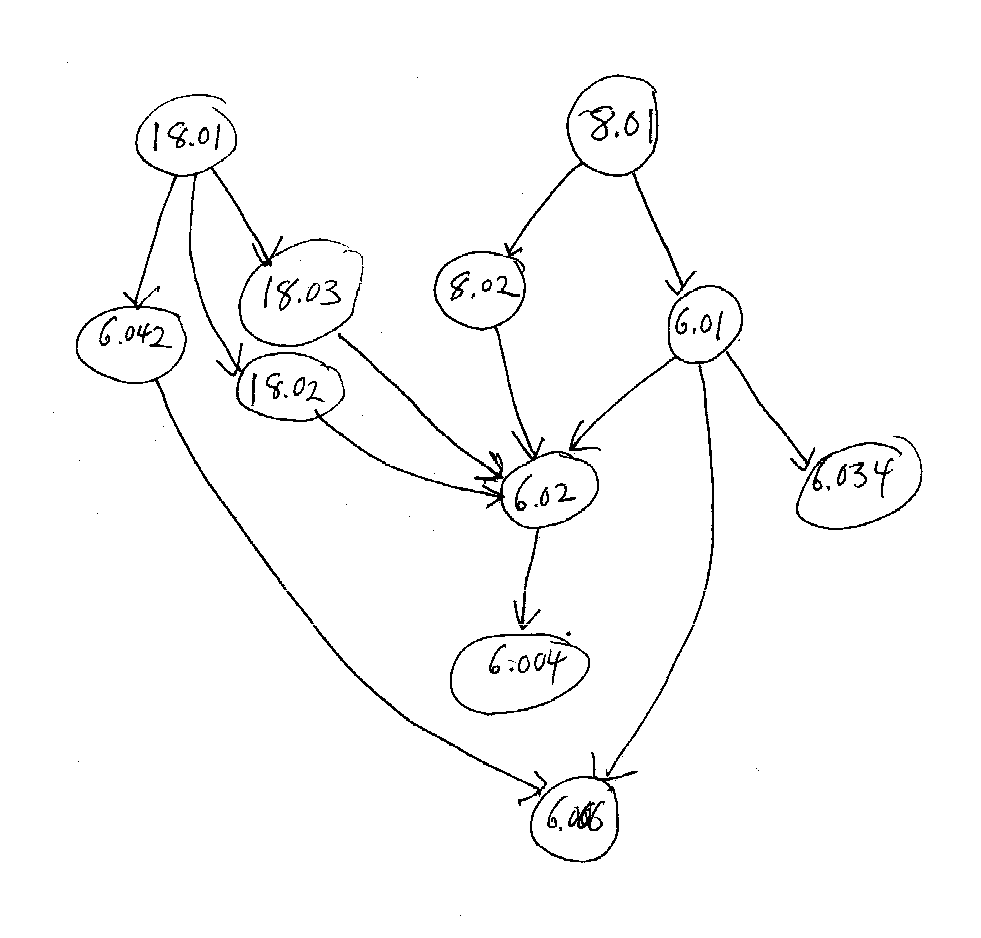
\includegraphics[height=4.0in]{prereq-poset-preview}
\end{center}

\end{solution}

\ppart Give an example of a collection of sets partially ordered by
the proper subset relation, $\subset$, that is isomorphic to (``same
shape as'') the prerequisite relation among MIT subjects from
part~\eqref{prereqtable}.

\begin{solution}
For each subject, $S$, let 
\[
\text{preset}(S) \eqdef \set{S' \suchthat S' \text{ is an indirect
    prerequisite of } S \QOR S' = S}.
\]
For example,
\[\begin{array}{|c|c|}\hline
\text{subject} & \text{preset}\\
\hline 
18.02   & \set{18.01, 18.02}\\
18.03   & \set{18.01, 18.03}\\
6.006   & \set{6.042, 18.01, 6.01, 8.01, 6.006}\\
\hline
\end{array}\]

Note that the ``$\QOR\ S' = S$'' clause is necessary: if we let the
set representing subject $S$ just be the indirect prerequisites of
$S$, then 18.02 and 18.03, for example, would be represented by the
same set, $\set{18.01}$.  Then the correspondence between subjects and
sets would no longer be a bijection, which is a requirement for
isomorphism.

\end{solution}


\begin{staffnotes}
Ask what would go wrong if the set corresponding to a subject
consisted only of its indirect prerequisites (that is, the subject
itself was not included in the corresponding set)?  18.01 and 6.042
illustrate the problem: they have the same indirect prerequisites, so
the correspondence between subjects and sets of indirect prerequisites
is not a bijection.
\end{staffnotes}

\ppart Explain why the \idx{empty relation} is a strict partial order
and describe a collection of sets partially ordered by the proper
subset relation that is isomorphic to the empty relation on five elements
---that is, the relation under which none of the five elements is
related to anything.

\begin{solution}
  An empty relation is always a partial order: it is \emph{vacuously}
  asymmetric and transitive.  It's not weak because it is not
  reflexive; in fact it's irreflexive.

  Letting the five elements be $1,2,3,4,5$, the recipe of mapping an
  element to its preimages under the relation, with the element itself
  thrown in, gives the five sets
  $\set{1},\set{2},\set{3},\set{4},\set{5}$.

  Of course any 5 sets none of which is contained in any of the others
  will also work, for example, all the size 4 subsets of
  $\set{1,2,3,4,5}$
\end{solution}

\ppart Describe a \emph{simple} collection of sets partially ordered
by the proper subset relation that is isomorphic to the "properly
contains'' relation, $\supset$, on $\power{\set{1, 2, 3,4}}$.

\begin{staffnotes}
If people get hung up on ``simple,'' explain that it means ``simpler
than the general approach of representing an element by the set of
elements less than or equal to it.''
\end{staffnotes}

\begin{solution}
  The standard inverse image solution involves sets of subsets.  A more
  elegant correspondence is to let each set $A \subseteq \set{1, 2, 3,4}$
  correspond to its complement.  That is,
\[
f(A) = \bar{A} \eqdef \set{1, 2, 3,4} - A.
\]
This works because $A \supset B$ iff $\bar{A} \subset \bar{B}$

\end{solution}

\begin{staffnotes}
Ask for a precise definition of isomorphism (without looking it up the
definition in the text).  You can give the hint that the definition of
isomorphism of partial orders is identical to the general definition
of isomorphism relations.

Here's Definition~\bref{relation-isomorphism}:
\begin{quote}

  A binary relation, $R$, on a set, $A$, is
  \term{isomorphic} to a relation, $S$, on a set $D$ iff there is a
  relation-preserving bijection from $A$ to $D$.  That is, there is
  bijection $f:A \to D$, such that for all $a,a' \in A$,
  \[
  a \mrel{R} a'\ \qiff\ f(a) \mrel{S} f(a').
  \]

\end{quote}

\end{staffnotes}

\eparts

\end{problem}

%%%%%%%%%%%%%%%%%%%%%%%%%%%%%%%%%%%%%%%%%%%%%%%%%%%%%%%%%%%%%%%%%%%%%
% Problem ends here
%%%%%%%%%%%%%%%%%%%%%%%%%%%%%%%%%%%%%%%%%%%%%%%%%%%%%%%%%%%%%%%%%%%%%

\endinput
